
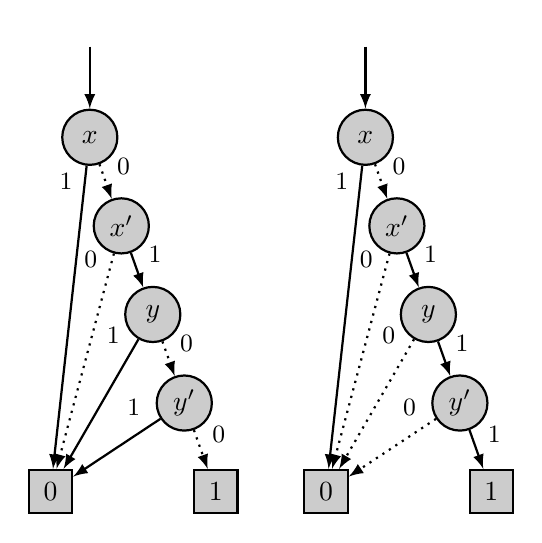
\begin{tikzpicture}[%
        costnode/.style={pos=0.6,rectangle,thick,solid,
                inner sep=2pt,draw,fill=white,text=black,font=\small},%
        decisionnode/.style={circle,thick,minimum size=4mm,
                inner sep=2pt,draw,fill=white!80!black,text=black,font=\normalsize},%
        xscale=2,yscale=1.5,>=latex]
    \begin{scope}
        \node[] (before) at (0,3.85) {}; % incoming edge_value
        \node[decisionnode, minimum size=0.7cm] (x) at (0,3) {$x$};
        \node[decisionnode, minimum size=0.7cm] (xp) at (0.2,2.25) {$x'$};
        \node[decisionnode, minimum size=0.7cm] (y) at (0.4,1.5) {$y$};
        \node[decisionnode, minimum size=0.7cm] (yp) at (0.6,0.75) {$y'$};
        \node[draw,thick,fill=white!80!black,rectangle, minimum size=0.55cm]
        (after0) at (-0.25,0) {{$0$}};
        \node[draw,thick,fill=white!80!black,rectangle, minimum size=0.55cm]
        (after1) at (0.8,0) {{$1$}};
        \draw[->, thick] (before) to (x);
        % x =>
        \draw[->, thick, dotted] (x) to[bend right=0,label distance=0mm,edge
        label={\small{$0$}},pos=0.6] (xp);
        \draw[->, thick] (x) to[bend left=0,label distance=0mm,edge
        label={\small{$1$}},swap,pos=0.1] (after0);
        % xp =>
        \draw[->, thick, dotted] (xp) to[bend right=0,label distance=0mm,edge
        label={\small{$0$}},swap,pos=0.1] (after0);
        \draw[->, thick] (xp) to[bend left=0,label distance=0mm,edge
        label={\small{$1$}},pos=0.6] (y);
        % y =>
        \draw[->, thick, dotted] (y) to[bend right=0,label distance=0mm,edge
        label={\small{$0$}},pos=0.6] (yp);
        \draw[->, thick] (y) to[bend left=0,label distance=0mm,edge
        label={\small{$1$}},swap,pos=0.1] (after0);
        % yp =>
        \draw[->, thick, dotted] (yp) to[bend right=0,label distance=0mm,edge
        label={\small{$0$}},pos=0.6] (after1);
        \draw[->, thick] (yp) to[bend left=0,label distance=0mm,edge
        label={\small{$1$}},swap,pos=0.1] (after0);
    \end{scope}
    \begin{scope}[xshift=1.75cm]
        \node[] (before) at (0,3.85) {}; % incoming edge_value
        \node[decisionnode, minimum size=0.7cm] (x) at (0,3) {$x$};
        \node[decisionnode, minimum size=0.7cm] (xp) at (0.2,2.25) {$x'$};
        \node[decisionnode, minimum size=0.7cm] (y) at (0.4,1.5) {$y$};
        \node[decisionnode, minimum size=0.7cm] (yp) at (0.6,0.75) {$y'$};
        \node[draw,thick,fill=white!80!black,rectangle, minimum size=0.55cm]
        (after0) at (-0.25,0) {{$0$}};
        \node[draw,thick,fill=white!80!black,rectangle, minimum size=0.55cm]
        (after1) at (0.8,0) {{$1$}};
        \draw[->, thick] (before) to (x);
        % x =>
        \draw[->, thick, dotted] (x) to[bend right=0,label distance=0mm,edge
        label={\small{$0$}},pos=0.6] (xp);
        \draw[->, thick] (x) to[bend left=0,label distance=0mm,edge
        label={\small{$1$}},swap,pos=0.1] (after0);
        % xp =>
        \draw[->, thick, dotted] (xp) to[bend right=0,label distance=0mm,edge
        label={\small{$0$}},swap,pos=0.1] (after0);
        \draw[->, thick] (xp) to[bend left=0,label distance=0mm,edge
        label={\small{$1$}},pos=0.6] (y);
        % y =>
        \draw[->, thick, dotted] (y) to[bend right=0,label distance=0mm,edge
        label={\small{$0$}},swap,pos=0.1] (after0);
        \draw[->, thick] (y) to[bend left=0,label distance=0mm,edge
        label={\small{$1$}},pos=0.6] (yp);
        % yp =>
        \draw[->, thick, dotted] (yp) to[bend right=0,label distance=0mm,edge
        label={\small{$0$}},swap,pos=0.1] (after0);
        \draw[->, thick] (yp) to[bend left=0,label distance=0mm,edge
        label={\small{$1$}},pos=0.6] (after1);
    \end{scope}
\end{tikzpicture}
